\documentclass[11pt]{article}

\usepackage{fullpage}
\usepackage{rotate}

\def\rootdir{../}

\usepackage{graphicx}
\usepackage{times}
\usepackage{multicol}
\usepackage{multirow}
\usepackage{latexsym}
\usepackage{url}
\usepackage{xspace}
\usepackage{verbatim}
\usepackage{booktabs}
\usepackage{fullpage}
\usepackage{fancyvrb}
\usepackage{color}
\usepackage{listings}
\usepackage{amsthm}
\usepackage{amsmath}
\usepackage{enumerate}
\usepackage{subfigure}
\usepackage[sectionbib]{bibunits}
\usepackage{hyperref}
\usepackage{rotating}
\usepackage{Tabbing}
\usepackage[all]{xy}
\usepackage[textsize=scriptsize,textwidth=1cm]{todonotes}

\newlength{\tab}
\setlength{\tab}{1em}
\setlength{\parindent}{0pt}
\setlength{\parskip}{6pt}
\setlength{\evensidemargin}{0.0cm}
\setlength{\oddsidemargin}{0.0cm}
\setlength{\textwidth}{16cm}
%  \setlength{\headsep}{0cm}
\setlength{\headheight}{0cm}
\setlength{\topmargin}{0cm}
\setlength{\textheight}{23cm}
\setlength{\itemsep}{0pt}
\setlength{\topsep}{0pt}


\definecolor{javared}{rgb}{0.6,0,0} % for strings
\definecolor{javagreen}{rgb}{0.25,0.5,0.35} % comments
\definecolor{javapurple}{rgb}{0.5,0,0.35} % keywords
\definecolor{javadocblue}{rgb}{0.25,0.35,0.75} % javadoc
\definecolor{javabackground}{rgb}{0.9,0.9,0.9}
\definecolor{javablack}{rgb}{0,0,0}

\lstset{language=Ada,
  backgroundcolor=\color{javabackground},
  basicstyle=\ttfamily\fontsize{10}{12}\selectfont,
  keywordstyle=\color{javablack}\bfseries,
  aboveskip={1.5\baselineskip},
  stringstyle=\color{javared},
  commentstyle=\color{javagreen},
  morecomment=[s][\color{javadocblue}]{/**}{*/},
  numbers=left,
  numberstyle=\tiny\color{black},
  frame=single,
  numbersep=10pt,
  stepnumber=1,
  tabsize=8,
  xleftmargin=0ex,
  xrightmargin=0ex,
  showspaces=false,
  showstringspaces=false,
  aboveskip=0.5ex
}

\newtheoremstyle{defstyle} % name of the style to be used
  {\parskip} % measure of space to leave above the theorem. E.g.: 3pt
  {\parskip} % measure of space to leave below the theorem. E.g.: 3pt
  {}% name of font to use in the body of the theorem
  {}% measure of space to indent
  {\bf}% name of head font
  {\\}% punctuation between head and body
  {.5em}% space after theorem head; " " = normal interword space
  {\thmname{#1}\thmnumber{ #2}~~ {\rm \thmnote{(#3)}}}% header

\newcommand{\tutorialtitle}[1]{
\begin{center}
\textbf{\sc SWEN90010: High Integrity Systems Engineering}\\[0.5ex]
\textbf{\sc Department of Computing and Information Systems}\\[0.5ex]
\textbf{\sc The University of Melbourne}\\[2ex]
\textbf{\large Workshop {#1}}
\end{center}
}


\newcommand{\tutorialsolutionstitle}[1]{
\begin{center}
\textbf{\sc SWEN90010: High Integrity Systems Engineering}\\[0.5ex]
\textbf{\sc Department of Computing and Information Systems}\\[0.5ex]
\textbf{\sc The University of Melbourne}\\[2ex]
\textbf{\large Workshop {#1} sample solutions}
\end{center}
}

\newcommand{\tobedone}[1]{\todo[inline,color=green!20!white]{\textbf{TODO:} #1}}

\newcommand{\tm}[1]{\todo[inline,color=yellow]{\textbf{Tim says:} #1}}


\newlength{\tab}
\setlength{\tab}{1em}
\setlength{\parindent}{0pt}
\setlength{\parskip}{6pt}
\setlength{\evensidemargin}{0.0cm}
\setlength{\oddsidemargin}{0.0cm}
\setlength{\textwidth}{16cm}
%  \setlength{\headsep}{0cm}
\setlength{\headheight}{0cm}
\setlength{\topmargin}{0cm}
\setlength{\textheight}{23cm}
\setlength{\itemsep}{0pt}
\setlength{\topsep}{0pt}


\definecolor{javared}{rgb}{0.6,0,0} % for strings
\definecolor{javagreen}{rgb}{0.25,0.5,0.35} % comments
\definecolor{javapurple}{rgb}{0.5,0,0.35} % keywords
\definecolor{javadocblue}{rgb}{0.25,0.35,0.75} % javadoc
\definecolor{javabackground}{rgb}{0.9,0.9,0.9}
\definecolor{javablack}{rgb}{0,0,0}

\lstset{language=Ada,
  backgroundcolor=\color{javabackground},
  basicstyle=\ttfamily\fontsize{10}{12}\selectfont,
  keywordstyle=\color{javablack}\bfseries,
  aboveskip={1.5\baselineskip},
  stringstyle=\color{javared},
  commentstyle=\color{javagreen},
  morecomment=[s][\color{javadocblue}]{/**}{*/},
  numbers=left,
  numberstyle=\tiny\color{black},
  frame=single,
  numbersep=10pt,
  stepnumber=1,
  tabsize=8,
  xleftmargin=0ex,
  xrightmargin=0ex,
  showspaces=false,
  showstringspaces=false,
  aboveskip=0.5ex
}


\begin{document}

\section*{Lecture aims}

 \begin{enumerate}
  
  \item Refresh knowledge of first-order predicate logic and set theory.

  \item Critique the use of formal modelling in software engineering, why it is used, what it is good for, what it is not good for.

  \item Read and write basic of Alloy state machines from informal requirements.

  \item Use Alloy operators to incrementally derive a specification.

 \end{enumerate}

\section*{Lecture plan}

\begin{enumerate}

 \item Background:

   \begin{enumerate}

   \item Overview of set theory, propositional logic, and predicate logic
     
   \item Important concepts: 
     
   \item Propositional logic: atomic propositions, conjunction, disjunction, implication, equivalence, negation, tautologies and contradictions
     
   \item Predicate logic: quantifiers (all, some, none, lone, one), predicates

   \item Relational calculus: sets as unary relaions, set membership, Cartesian product, union, intersection, difference, dot join, box join, relations, functions (total and partial), function override,  domain \& range restriction.

   \end{enumerate}
 
 \item Motivation for formal, model-based specification:

 \begin{enumerate}

 \item Example: sorting a list; binary search

 \item What is formal specification? What is model-based specification?
   
 \item Why use formal specification? 

 \item Why use set theory and predicate logic?
   
 \item Cost savings: no ambiguity, solve problems up front, easier to implement, \emph{proof}, post-release costs (more mistakes made \emph{and found} in specification).
   
 \item Objections: too hard for ``average'' programmer

 \end{enumerate}

 \item Alloy

 \begin{enumerate}

  \item Motivation: based on Z which is well-known, highly-used language; intuitive notation, state-of-the-art tool support. Loads and loads of examples.

  \item Alloy = logic + language + analysis; analysis is NOT proof, but counterexample driven.

  \item Basic: modules. 

  \item Running example of the PassBook

  \item Signatures are basically types.

  \item Facts hold over entire signature space

  \item Predicates and functions; we use these to specify \emph{operations}.

  \item Assertions state properties about model; can be checked but also serve to help understand the model itself. 

 
  \item Incremental specification: abstract state machines (state, inv, init, operations); preconditions and postconditions, inclusion (building up from components using conjunction and disjunction), assertions (invariant preservation).

 \end{enumerate}

 \item Formal development process (see figure below).

 \item V\&V: animation, model checking, review!!, and proof.

 \item Example: Needham-Schroeder protocol mutual authentication. Considered correct for many years, but man-in-the-middle attach was possible, and found using formal proof.

 \item Example: modal checking -- NASA's use of checking high-level models to find deadlock.

 \item Show Bill Gates quote about proof (without the name!) below.

 \item Example proof: storage tank in chemical plant does not overflow.


\end{enumerate}

\pagebreak

\begin{center}
\includegraphics[scale=0.8]{./figures/CICS-graph}
\end{center}

\pagebreak

\begin{center}
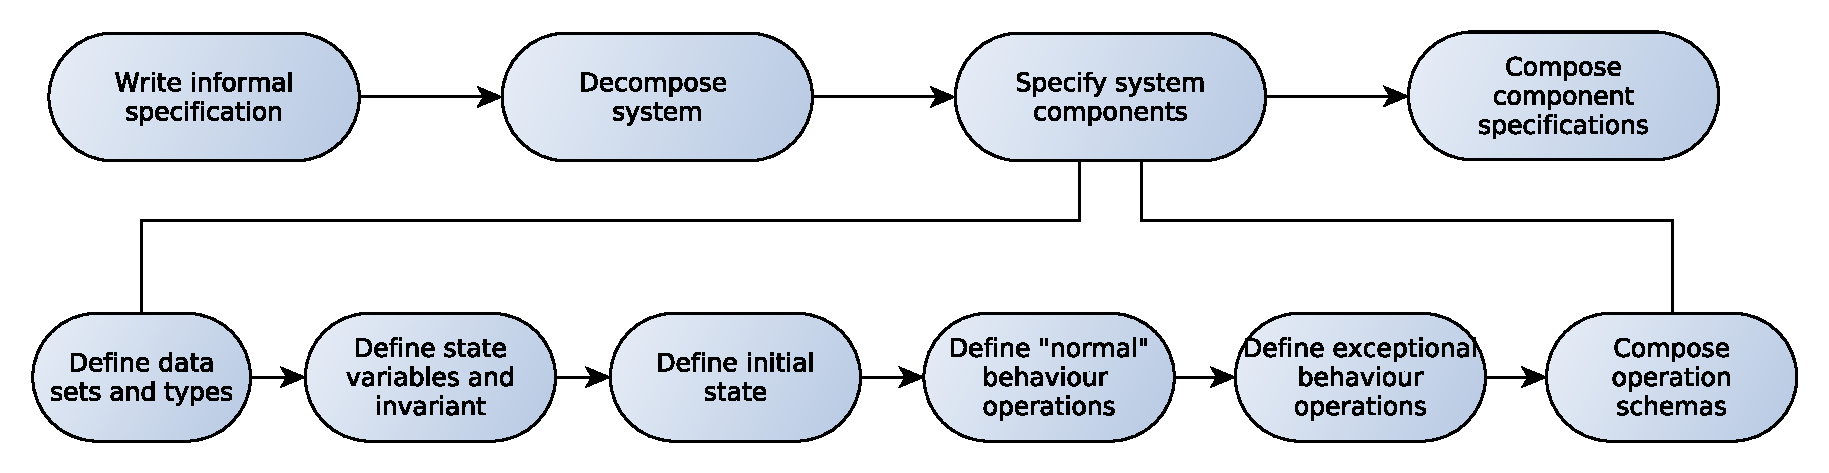
\includegraphics[scale=0.6,angle=90]{./figures/specification-process}
\end{center}

\pagebreak

~

~

~

~

~

~

~


\begin{quote}
``Things like even software verification, this has been the Holy Grail of computer science for many decades but now in some very key areas, for example, driver verification we're building tools that can do actual proof about the software and how it works in order to guarantee the reliability." 
\end{quote}

\newpage

\alloyfile{}{\rootdir/specification/code/lastpass.als}

\newpage

\alloyfile{}{\rootdir/specification/code/expanded_lastpass.als}


\end{document}  

% LocalWords:  init PreFill PostFill FillOK GSM de Franche
